\documentclass[a4paper]{scrartcl}
\usepackage[english]{babel}
\usepackage[utf8]{inputenc}
\usepackage[T1]{fontenc}
\usepackage{ae}
\usepackage[bookmarks,bookmarksnumbered,colorlinks=true]{hyperref} % http://ctan.org/pkg/hyperref
\usepackage{nameref}
\usepackage{comment} % for block commenting
\usepackage{graphicx}
% \usepackage[export]{resources/adjustbox}
\usepackage{float}
\graphicspath{{./images/}}
\usepackage{todonotes} % use temporary for todo notes
\usepackage[nonumberlist,acronym,toc,section]{glossaries} % must be the last package to include

% glossary
\makeglossaries
% Remove trailing dot
\renewcommand*{\glspostdescription}{}

%
% Glossary entries
%

\newglossaryentry{graphioli}{name=Graphioli,
description={A fancy name that combines \glspl{graph} with filled pasta.},
plural={Graphioli}}

\newglossaryentry{graph}{name=graph,
description={A (abstract) set of objects provided with binary relations.\\The objects of a graph are called \glspl{vertex} and are represented by nodes in the visualization. The relations are called \glspl{edge} and are represented by (in our case straight) lines between the respective vertices in a visualized graph.\todo{Passt so?}}}

\newglossaryentry{edge}{name=edge,
description={see \emph{\gls{graph}}}}

\newglossaryentry{vertex}{name=vertex,
description={see \emph{\gls{graph}}},
plural={vertices}}

\newglossaryentry{planar}{name=planar,
description={A \emph{planar} \gls{graph} is a graph that can be structure-preservingly redrawn in a way that no \glspl{edge} intersect.},
plural={planar}}

\newglossaryentry{planarity}{name=planarity,
description={see \emph{\gls{planar}}},
plural={planarities}}

\newglossaryentry{api}{name=application programming interface (API),
description={Set of routines and tools providing \gls{program} blocks, which are put together by a third-party programmer to ensure consistency with an existing program or \gls{framework}.}}

\newglossaryentry{gui}{name=graphical user interface (GUI),
description={\Gls{program} interface that uses a computer's graphical capabilities to provide easy access and handling for the program. It replaces the command-line based access.},
plural={graphical user interfaces (GUI)}}

\newglossaryentry{framework}{name=framework,
description={A layered structure indicating what kind of applications can or should be built and how they would interrelate. It specifies interfaces and reusable \glspl{program} that form the basis for such an application.}}

\newglossaryentry{java}{name=Java,
description={Java is a widely spread programming language originally developed by Sun Microsystems and released in 1995. Applications developed with Java are compiled into bytecode that runs on basically every system that has a \Gls{jvm} installed.},
plural={Java}}

\newglossaryentry{jvm}{name=Java Virtual Machine (JVM),
description={A virtual machine that can execute \Gls{java} byte code. Thus, the execution component of the Java platform.},
plural={Java Virtual Machines (JVM)}}

\newglossaryentry{jdk}{name=Java Development Kit (JDK),
description={A collection of programming tools for \Gls{java} developers.},
plural={Java Development Kit (JDK)}}

\newglossaryentry{jre}{name=Java Runtime Environment,
description={see \emph{\gls{jvm}}}}

\newglossaryentry{javadoc}{name=Javadoc,
description={Javadoc is a tool for generating API documentation in HTML format from doc comments in source code.\footnote{From Oracle, self-definition}},
plural={Javadoc}}

\newglossaryentry{customer}{name=customer,
description={A party that receives a copy of the created \gls{software} in order to use it for own implementations. The customer of this \gls{framework} will be the \gls{developer}.}}

\newglossaryentry{computer-game}{name=computer game,
description={An electronic game that requires the \gls{player}['s] interaction to influence its course of events. Such a game usually bases on graphical feedback.}}

\newglossaryentry{game}{name=game,
description={The implementation of a \gls{computer-game} that requires the usage of this \gls{framework}.}}

\newglossaryentry{network}{name=network,
description={A group of connected computers that are able to communicate and share data, e.g. for synchronizing \gls{game} statuses.}}

\newglossaryentry{tutorial}{name=tutorial,
description={Instructional document that provides step by step information about a specific topic or \gls{workflow}, e.g. how to start implementing your own \gls{game} using this \gls{framework}.}}

\newglossaryentry{editor}{name=editor,
description={see \emph{\gls{level-editor}}}}

\newglossaryentry{level-editor}{name=level editor,
description={An interface that lightens the \gls{developer}['s] workload at creating new levels.}}

\newglossaryentry{level}{name=level,
description={A stage of the current \gls{game}.}}

\newglossaryentry{player}{name=player,
description={One who plays one of the \glspl{game} developed by a \gls{developer} using this \gls{framework}.}}

\newglossaryentry{developer}{name=developer,
description={Someone who designs and implements \glspl{game} using the {\graphioli} framework.}}

\newglossaryentry{undo}{name=undo,
description={To restore a previous condition, e.g. a \gls{savegame} or the previous step in the \gls{level-editor}.}}

\newglossaryentry{redo}{name=redo,
description={Opposite of \emph{\gls{undo}}.}}

\newglossaryentry{four-color-theorem}{name=four color theorem,
description={In mathematics, the \emph{four color theorem} states that, given any separation of a plane into contiguous areas, no more than four colors are required to color these areas in a way that no two \gls{adjacent} areas have the same color.},
plural={four color theorem}}

\newglossaryentry{adjacent}{name=adjacent,
description={Two \glspl{vertex} connected by an \gls{edge} are called \emph{adjacent}.},
plural={adjacent}}

\newglossaryentry{program}{name=program,
description={see \emph{\gls{computer-program}}}}

\newglossaryentry{savegame}{name=savegame,
description={A data file that contains information about a current \gls{game} state and is created when saving a game. It allows the \gls{player} to jump to a previously reached level.}}

\newglossaryentry{computer-program}{name=computer program,
description={A sequence of instructions that a computer can interpret and execute.}}

\newglossaryentry{software}{name=software,
description={An organized collection of data and instructions for computers, that is used to accomplish specific tasks.\\A piece of software can consists of a single \gls{program} or a package of programs closely working together. Usually software is bundled with associated documentation.}}

\newglossaryentry{workflow}{name=workflow,
description={The sequence of administrative, technical, or other processes through which a \gls{software} project passes from initiation to completion.}}

\newglossaryentry{user}{name=user,
description={The \emph{user} of a \gls{software} is everybody how starts the \gls{program} in order to fulfill specified tasks.\\The user of this framework is the \gls{developer}, whereas the user of the final \gls{game} is the \gls{player} (see \ref{REF:HOW-TO-READ}).}}

\newglossaryentry{git}{name=Git,
description={A distributed revision control and source code management system developed by \emph{Linus Torvalds}. Every Git working directory is a full-fledged repository with complete history and full revision tracking capabilities, not dependent on network access or a central server.\footnote{From Wikipedia: Git (software), 08/05/2012}},
plural={Git}}

\newglossaryentry{eclipse}{name=Eclipse,
description={An open development platform comprised of extensible frameworks, tools and runtimes for building, deploying and managing software across the lifecycle.\footnote{From Eclipse project, self-definition}},
plural={Eclipse}}

\newglossaryentry{artificial-intelligence}{name=artificial intelligence (AI),
description={An intelligent system that perceives its environment and takes actions that maximize its chances of success.\footnote{Russell, Stuart J.; Norvig, Peter: Artificial Intelligence: A Modern Approach (2003, 2nd ed.)}\\An algorithm that tries to defeat its human counter-\glspl{player} in a \glspl{computer-game} could be referred to as \emph{artificial intelligence}.}}

\newglossaryentry{depth-first-search}{name=depth-first search (DFS),
description={An \gls{algorithm} for traversing or searching a \gls{graph}, starting at a selected root \gls{vertex} and exploring as far as possible along each branch before backtracking.\footnote{From Wikipedia: Breadth-first search, 08/05/2012}},
plural={depth-first searches (DFS)}}

\newglossaryentry{breadth-first-search}{name=breadth-first search (BFS),
description={An \gls{algorithm} for traversing or searching a \gls{graph}, starting at a selected root \gls{vertex} and inspecting all its neighboring vertices.},
plural={breadth-first searches (BFS)}}

\newglossaryentry{path}{name=path,
description={A sequence of \glspl{vertex} of a \gls{graph}.}}

\newglossaryentry{algorithm}{name=algorithm,
description={Procedure or set of (mathematical) rules for solving a problem in a finite number of steps, especially by a computer.}}

\newglossaryentry{library}{name=library,
description={A collection of resources used to develop \gls{software}. These may include pre-written code and subroutines, classes, values or type specifications.},
plural={libraries}}

\newglossaryentry{opensuse}{name=openSUSE,
description={A free and \Gls{linux}-based operating system.\footnote{From openSUSE Project, self-definition}},
plural={openSUSE}}

\newglossaryentry{linux}{name=Linux,
description={An alternative and open-source operating system for personal computers and servers.},
plural={Linuces}}

\newglossaryentry{metalanguage}{name=metalanguage,
description={Any (technical) language used to describe and define an implementation of a \gls{game} in the \gls{framework}. It substitutes the \Gls{java}-based programming of that implementation and can be parsed by the framework.}}

\newglossaryentry{mvc}{name=Model-View-Controller (MVC),
description={A design pattern for computer user interfaces describing the structural subdivision into the components `Model', `View' and `Controller'.},
plural={Model-View-Controllers (MVC)}}

\newglossaryentry{chat}{name=online chat,
description={A communication system over the internet.}}

%
% Acronyms
%

\newacronym{GUI}{GUI}{graphical user interface\protect\glsadd{gui}}

\newacronym{API}{API}{application programming interface\protect\glsadd{api}}

\newacronym{JVM}{JVM}{Java Virtual Machine\protect\glsadd{jvm}}

\newacronym{JDK}{JDK}{Java Development Kit\protect\glsadd{jdk}}

\newacronym{AI}{AI}{artificial intelligence\protect\glsadd{artificial-intelligence}}

\newacronym{DFS}{DFS}{depth-first search\protect\glsadd{depth-first-search}}

\newacronym{BFS}{BFS}{breadth-first search\protect\glsadd{breadth-first-search}}

\newacronym{MVC}{MVC}{Model-View-Controller\protect\glsadd{mvc}}

\newacronym{IDE}{IDE}{integrated development environment}

\newacronym{ID}{ID}{identification}

\author{Graphioli}

\begin{document}

\begin{titlepage}
\begin{center}
\fontsize{40}{50}\selectfont
        \vfill
        \textsc{Graphioli}
		\vfill
        \textsc{Functional Specification Document}
        \vfill
\LARGE
PSE SS 2012
  \vfill
 \newpage
 
 \null
 \vfill
 
 Praxis der Softwareentwicklung -- SS 2012 \\
 
  \Large
  Development of a Framework for Graph Games \\
  \medskip
  \vspace{2cm}
  
    Martin Dinh $\cdot$ Ole Fortmann $\cdot$ Leon Hielscher \\ Johannes Schäfer $\cdot$ Jack Unseld
  \vspace{2cm} \\
  \today
\end{center}

  \vfill

\end{titlepage}
\tableofcontents
\clearpage

\makeatletter
    \newcommand*{\textlabel}[2]{%
        \edef\@currentlabel{#1}% Set target label
        \phantomsection% Correct hyper reference link
        #1\label{#2}% Print and store label
    }
\makeatother

%%% proper nouns
\newcommand{\graphioli}{\textsc{Graphioli}}
\newcommand{\twixt}{\textsc {TwixT}}
\newcommand{\graphcoloring}{\textsc {Graph-Coloring}}

\section{Introduction}
Games premised on \gls{graph} algorithms have always been played as a pastime. Mostly without the knowledge about the underlying mathematical theories, which are – of course – not always relevant for clearing level after level. While two humans playing a graph game usually agree on the eventuation of one player winning the game, the same game on a computer must be computed to declare one player the winner.\\

This is where Graphioli takes effect. The java framework simplifies the process of developing graph-based computer games by providing an straightforward, intuitive library that allows its user to focus the effort to the game's logical implementation. Recurring and redundant operations, algorithms and codings will be taken care of by Graphioli.\\

Products based on Graphioli will be well-structured, lightweight in terms of code size and easy to maintain.
\section{Objectives}
\subsection{Mandatory criteria}
\subsubsection{Framework}
The framework provides rudimental functions that either all or the most games need. Such as creating new graphs from specifications and visualizing and manipulating existing graphs.\par
These graphs consist of \glspl{edge} and \glspl{vertice} that themselves are equipped with parameters. Parameters for edges are at least style (background color, border color, background image, size), coordinates, weight, sorting, \Gls{id}. Parameters that are related to vertices are at least weight, length and direction.\par
Furthermore the framework lightens a \gls{developer}['s] workload by providing access to reoccuring basic graph algorithms. These include path recognition (depth-first search, breadth-first search) and Dijkstra.\par
\emph{Graphioli} will offer interfaces for creating multiplayer modes so that two \glspl{player} are able to play against each other on the same computer sharing the same peripherals.\par
Games can be saved and restored by their user at a later time without losing \gls{level} stats.\par
In order to facilitate easy implementations, \emph{Graphioli} comes with elaborate \Gls{Javadoc} documentation for the viewpoint of the developer using the framework.\par


\subsubsection{GUI: Game-Explorer}
The Game-Explorer is a graphical interface that builds the main contact point with the framework for a player. Without knowledge about the background of framework and implemented game logic, the player is still able to start and restart games from a list of available or previously saved games.\par
For that reason, the Game-Explorer displays information to every game, such as title, description and a static screenshot. It comes with a \emph{START} button and a \emph{HELP} button for details about the rules and operability of the specific game.\par
The list of available games is dynamically created when the Game-Explorer starts. It reads a subfolder for legally specified games that are represented by a class that inherits from the frameworks game scaffold.

\subsubsection{Games}
\subsubsection{Graph coloring}
tbc.\par

\subsubsection{TwixT}
tbc.\par

\subsection{Facultative criteria}
\subsubsection{Framework}
\subsubsection{GUI: Game-Explorer}
\subsubsection{Games}

\subsection{Excluded criteria}
\section{Product usage}
The \gls{framework} serves as a \Gls{java} \gls{library} to easily implement \gls{graph} games. It provides a number of important, general functions and algorithms which allows the \gls{game-developer} to focus mainly on the game's logic.

\subsection{Scope}
The product shall be used to implement graph games on Java basis. It already contains a \gls{GUI} to display and interact with the graphs and several algorithms to relieve the coding work of potential game developer.

\subsection{Target}
The product helps graph game developer to easily develop their own graph games. While simply using the framework's general functions and \gls{GUI} they can mainly focus on their game's logic. \\
The framework mainly targets game developers who want to start immediately creating their own graph games without bothering to implement several algorithms or the \gls{GUI} beforehand.
\section{Product environment}

\subsection{Architecture}

\subsection{Software}
\begin{itemize}
\item Theoretical independence of platforms (Java) (optimally Linux Suse 11.3)
\item JRE, JDK
\item Text editor for coding
\end{itemize}

\subsection{Hardware}
\begin{itemize}
\item Input device (mouse (-pad), keyboard)
\item Output device (monitor)
\end{itemize}
Optimally:
\begin{itemize}
\item Intel E7200@2.66 Ghz
\item 4GB RAM
\end{itemize}
\section{Product functionalities}
\subsection{Functional requirements}

%%%%%%%%%%% Framework %%%%%%%%%%%

\subsubsection{Graphioli Framework}
\begin{tabular}{{c}{l}}
    \hline
    {\bf Functions} & {\bf Description} \\ \hline
	\ref{FR:010} & Add/Remove/Move nodes/vertices \\ 
	\ref{FR:020} & Nodes/Edges have attributes \\ 
	\ref{FR:030} & Find shortest path \\
	\ref{FR:040} & Check for planarity \\
	\ref{FR:050} & Display games with graphical user interface \\
	\ref{FR:060} & Print planar graphs \\
	\ref{FR:070} & Play as single player or against another player \\ 
	\ref{FR:080} & Timer \\ \hline
\end{tabular}

\vspace{.5cm}

\begin{description}
  	\item[/FR010/\label{FR:010}] {\bf Add/Remove/Move nodes/edges}  \hfill \\
	With the Graphioli frameworks the developer can do all basic graph operations. Nodes can be added to either a given graph or to initiate a new graph. Nodes can be removed and moved; in either case the edges will be removed or moved accordingly. In addition to adding, removing and moving nodes, the developer can also connect two given nodes with each other, and remove edges between nodes.
	\item[/FR020/\label{FR:020}] {\bf Nodes/Edges have attributes}  \\
	Each and every node and edge will have a set of attributes. The developer can completely change the appearance of a node by replacing the default icon with any graphic or by changing its color, stroke, or size. Additionally each node will have its own coordinates, its own weight, and an unique identification as attributes. Edges have attributes of their own, which the developer can set. An edge can have a weight, a length, and a direction.
	\item[/FR030/\label{FR:030}] {\bf Find shortest path}  \\
	The Graphioli framework implements algorithms to find the shortest path within a given graph.
	\item[/FR040/\label{FR:040}] {\bf  Check for planarity}  \\
	For a given graph, it is possible to verify, if an edge between two given unconnected nodes exists, so that the resulting graph is planar.
 	\item[/FR050/\label{FR:050}] {\bf Display games with graphical user interface}  \\
 	The graphical user interface \nameref{FR:game-explorer} can display all graph games, which where implemented using the Graphioli Framework.
	\item[/FR060/\label{FR:060}] {\bf Print planar graphs}  \\
  	With \ref{FR:010} and \ref{FR:020} the developer is able to draw a two-dimensional graph with a set of given nodes and edges.
	\item[/FR070/\label{FR:070}] {\bf Play as single player or against another player}  \\
	The Graphioli frameworks enables the developer to easily implement both single and multiplayer modes.
	\item[/FR080/\label{FR:080}] {\bf Timer} \\
	A timer function exists, which the developer can implement within his games.
\end{description}

%%%%%%%%%%% Explorer %%%%%%%%%%%

\subsubsection{Game-Explorer}\label{FR:game-explorer}
\begin{tabular}{{c}{l}}
    \hline
    {\bf Functions} & {\bf Description} \\ \hline
	\ref{FR:090} & Manage games \\
	\ref{FR:100} & Start games \\
	\ref{FR:110} & See game instructions \\
	\ref{FR:120} & Display description and image \\
	\ref{FR:130} & Load new games \\ \hline
\end{tabular}

\vspace{.5cm}

\begin{description}
  	\item[/FR090/\label{FR:090}] {\bf Manage games} \hfill \\
  	Managing games, which where implemented using the Graphioli framework is an easy task with the `Game-Explorer'. The `Game-Explorer' is the centerpiece for all games. It combines the games within one window and lets the player select a game to play. Every game is saved in a subfolder within the `Game-Explorer' directory.
 	\item[/FR100/\label{FR:100}] {\bf Start games}  \\
 	Once a game is selecting in the menu, the player can start a game by pressing the `Start' button.
	\item[/FR110/\label{FR:110}] {\bf See game instructions}  \\
  	A tutorial or instruction file for each game (provided by the developer), can be viewed by clicking the `Help' button, which opens up a new window with the instruction/tutorial.
	\item[/FR120/\label{FR:120}] {\bf Display description}  \\
	When a game is selected the `Game-Explorer' will display an image and a description of the game, which both are provided by the developer.
	\item[/FR130/\label{FR:130}] {\bf Load new games} \\
	The `Game-Explorer' can be extended with new games. Therefore a `Load' button exists, where the player can choose from a list of games. Once a game is added, a new menu entry will be displayed within his `Game-Explorer' list of games. Which then can be selected to be played. Games that are already in the `Game' folder will be automatically loaded into the game list.
\end{description}

%%%%%%%%%%% GAMES %%%%%%%%%%%

\subsubsection{Implemented Games}
\begin{tabular}{{c}{l}}
    \hline
    {\bf Functions} & {\bf Description} \\ \hline
	\ref{FR:140} & Save games \\
	\ref{FR:150} & Load games \\
	\ref{FR:160} & Pause games \\
	\ref{FR:170} & Restart game \\
	\ref{FR:180} & Undo move \\
	\ref{FR:190} & Redo move \\
	\ref{FR:200} & Take screenshots \\ \hline
\end{tabular}

\vspace{.5cm}

\begin{description}
  	\item[/FR140/\label{FR:140}] {\bf Save games}  \hfill \\
  	A started and running game can be saved by clicking the `Menu' button in the navigation bar and selecting `Save'.
 	\item[/FR150/\label{FR:150}] {\bf Load games}  \\
 	A saved game can easily be resumed by starting the game and, depending on the implementation of the developer, either a window pops up, which offers the option to load a saved game, or by clicking the `Menu' button and selecting `Load'.
	\item[/FR160/\label{FR:160}] {\bf Pause games}  \\
	While playing in single mode, a game can be paused anytime. In multiplayer mode a game can only be paused, if both parties agree to halt the game. A game can be paused by going into the `Menu' and selecting `Game' then `Take Screen'.
	\item[/FR170/\label{FR:170}] {\bf Restart game}  \\
	A game can be restarted anytime during a single mode game. Like \ref{FR:150} a game can only be restarted in multiplayer mode, if both parties agree upon it. Restarting can be accomplished by clicking `Restart' in the navigation bar under `Game'.
	\item[/FR180/\label{FR:180}] {\bf Undo move}  \\
	Depending on the implementation of the developer, a player can either undo infinite amount of recent moves or a limited amount of moves. A move can be reverted like all the other game operations, by clicking the `Menu' item in the navigation bar and selecting `Undo'.
	\item[/FR190/\label{FR:190}] {\bf Redo move} \\
	If a player accidentally hit the `Undo' button or decides that the undo was not a wise choice, he can redo all `undoes' again by clicking the `Menu' item and selecting `Redo'.
	\item[/FR200/\label{FR:200}] {\bf Take screenshots} \\
	A player can take a screenshot of his current game anytime during a running game. To take a screenshot, the player will have to go into the game menu and select `Take Screen'. All screenshots will be saved in a subfolder within the game folder.
\end{description}

% Non-functional requirements %

\subsection{Non-functional requirements}

%%%%%%%%%%% Framework %%%%%%%%%%%

\subsubsection{Graphioli Framework}
\begin{tabular}{{c}{l}}
    \hline
    {\bf Functions} & {\bf Description} \\ \hline
	\ref{NFR:010} & Simple usage \\
	\ref{NFR:020} & Documentation in detail \\ \hline
\end{tabular}

\vspace{.5cm}

\begin{description}
  	\item[/NFR010/\label{NFR:010}] {\bf Simple implementation}  \hfill \\
	The Graphioli framework can be easily understood by the developer after a short period of induction. The induction should not take longer than one day for the developer to fully be able to work with the framework. \\
	\item[/NFR020/\label{NFR:020}] {\bf Documentation in detail} \\
	The framework has an simple to understand and easy accessible documentation. Each class, method will be described in detail with all attributes, parameters, and usage.
\end{description}

%%%%%%%%%%% GAMES %%%%%%%%%%%
\subsubsection{Graphioli Framework}
\begin{tabular}{{c}{l}}
    \hline
    {\bf Functions} & {\bf Description} \\ \hline
	\ref{NFR:030} & Crashes \\
	\ref{NFR:040} & Short loading time \\ 
	\ref{NFR:050} & Security \\ \hline
\end{tabular}

\vspace{.5cm}

\begin{description}
  	\item[/NFR030/\label{NFR:030}] {\bf Crashes}  \hfill \\
	Games implemented with the Graphioli framework will not crash more often than once per 10.000 uses. \\
	\item[/NFR040/\label{NFR:040}] {\bf Short loading time} \\
	The loading time of the implemented games will be shorter than 5 seconds. \\
	\item[/NFR050/\label{NFR:050}] {\bf Security} \\
	All the games implemented with the Graphioli framework will have none security vulnerability.
\end{description}


\section{Product data}

\begin{tabular}{{c}{l}} \hline
    {\bf Data} & {\bf Description} \\ \hline
    \ref{PD:010} & \ref{PD:T010} \\
    \ref{PD:020} & \ref{PD:T020} \\
    \ref{PD:030} & \ref{PD:T030} \\
    \ref{PD:040} & \ref{PD:T040} \\ \hline
\end{tabular}

\begin{description}
	\item[\textlabel{/PD010/}{PD:010}] {\bf \textlabel{Game-explorer}{PD:T010}}
	In our game explorer there is a short description and screenshot of each game possible.
	\item[\textlabel{/PD020/}{PD:020}] {\bf \textlabel{Tutorial}{PD:T020}}
	The game developers provide an explanation and/or tutorial of their implemented graph games.
	\item[\textlabel{/PD030/}{PD:030}] {\bf \textlabel{Default designed levels (graphs)}{PD:T030}}
	Some games require different graphs each time they are played. The game developer creates possible graphs to play his game which are then loaded.
	\item[\textlabel{/PD040/}{PD:040}] {\bf \textlabel{Savegames}{PD:T040}}
	Players are able to, if implemented by the developer, save their current state of the game.
\end{description}
\section{System model}

\begin{figure}[h]
	\centering
	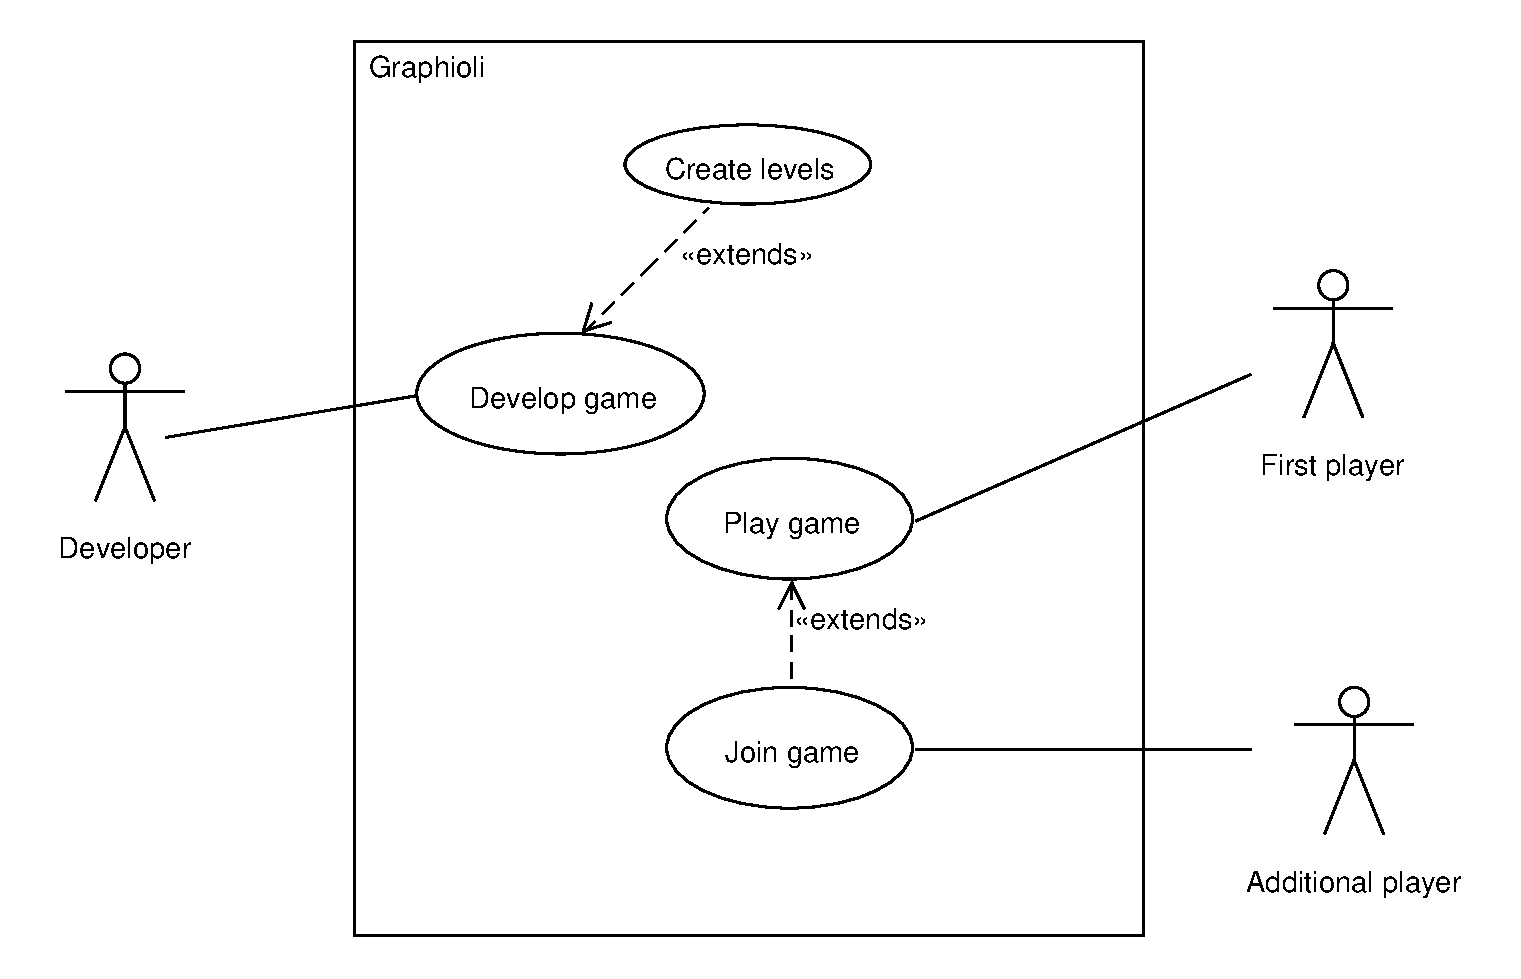
\includegraphics[max width=\linewidth]{usecase.pdf}
	\caption{Use case diagram}
	\label{img:UCD}
\end{figure}

The use case diagram depicts (\ref{img:UCD}) the  way of users (game developers or players) interacting with the framework in general. The follwoing scenarios depict more specific usages.
\subsection{Scenarios}

\subsubsection{Game development and usage}
\begin{figure}[h!]
	\centering
	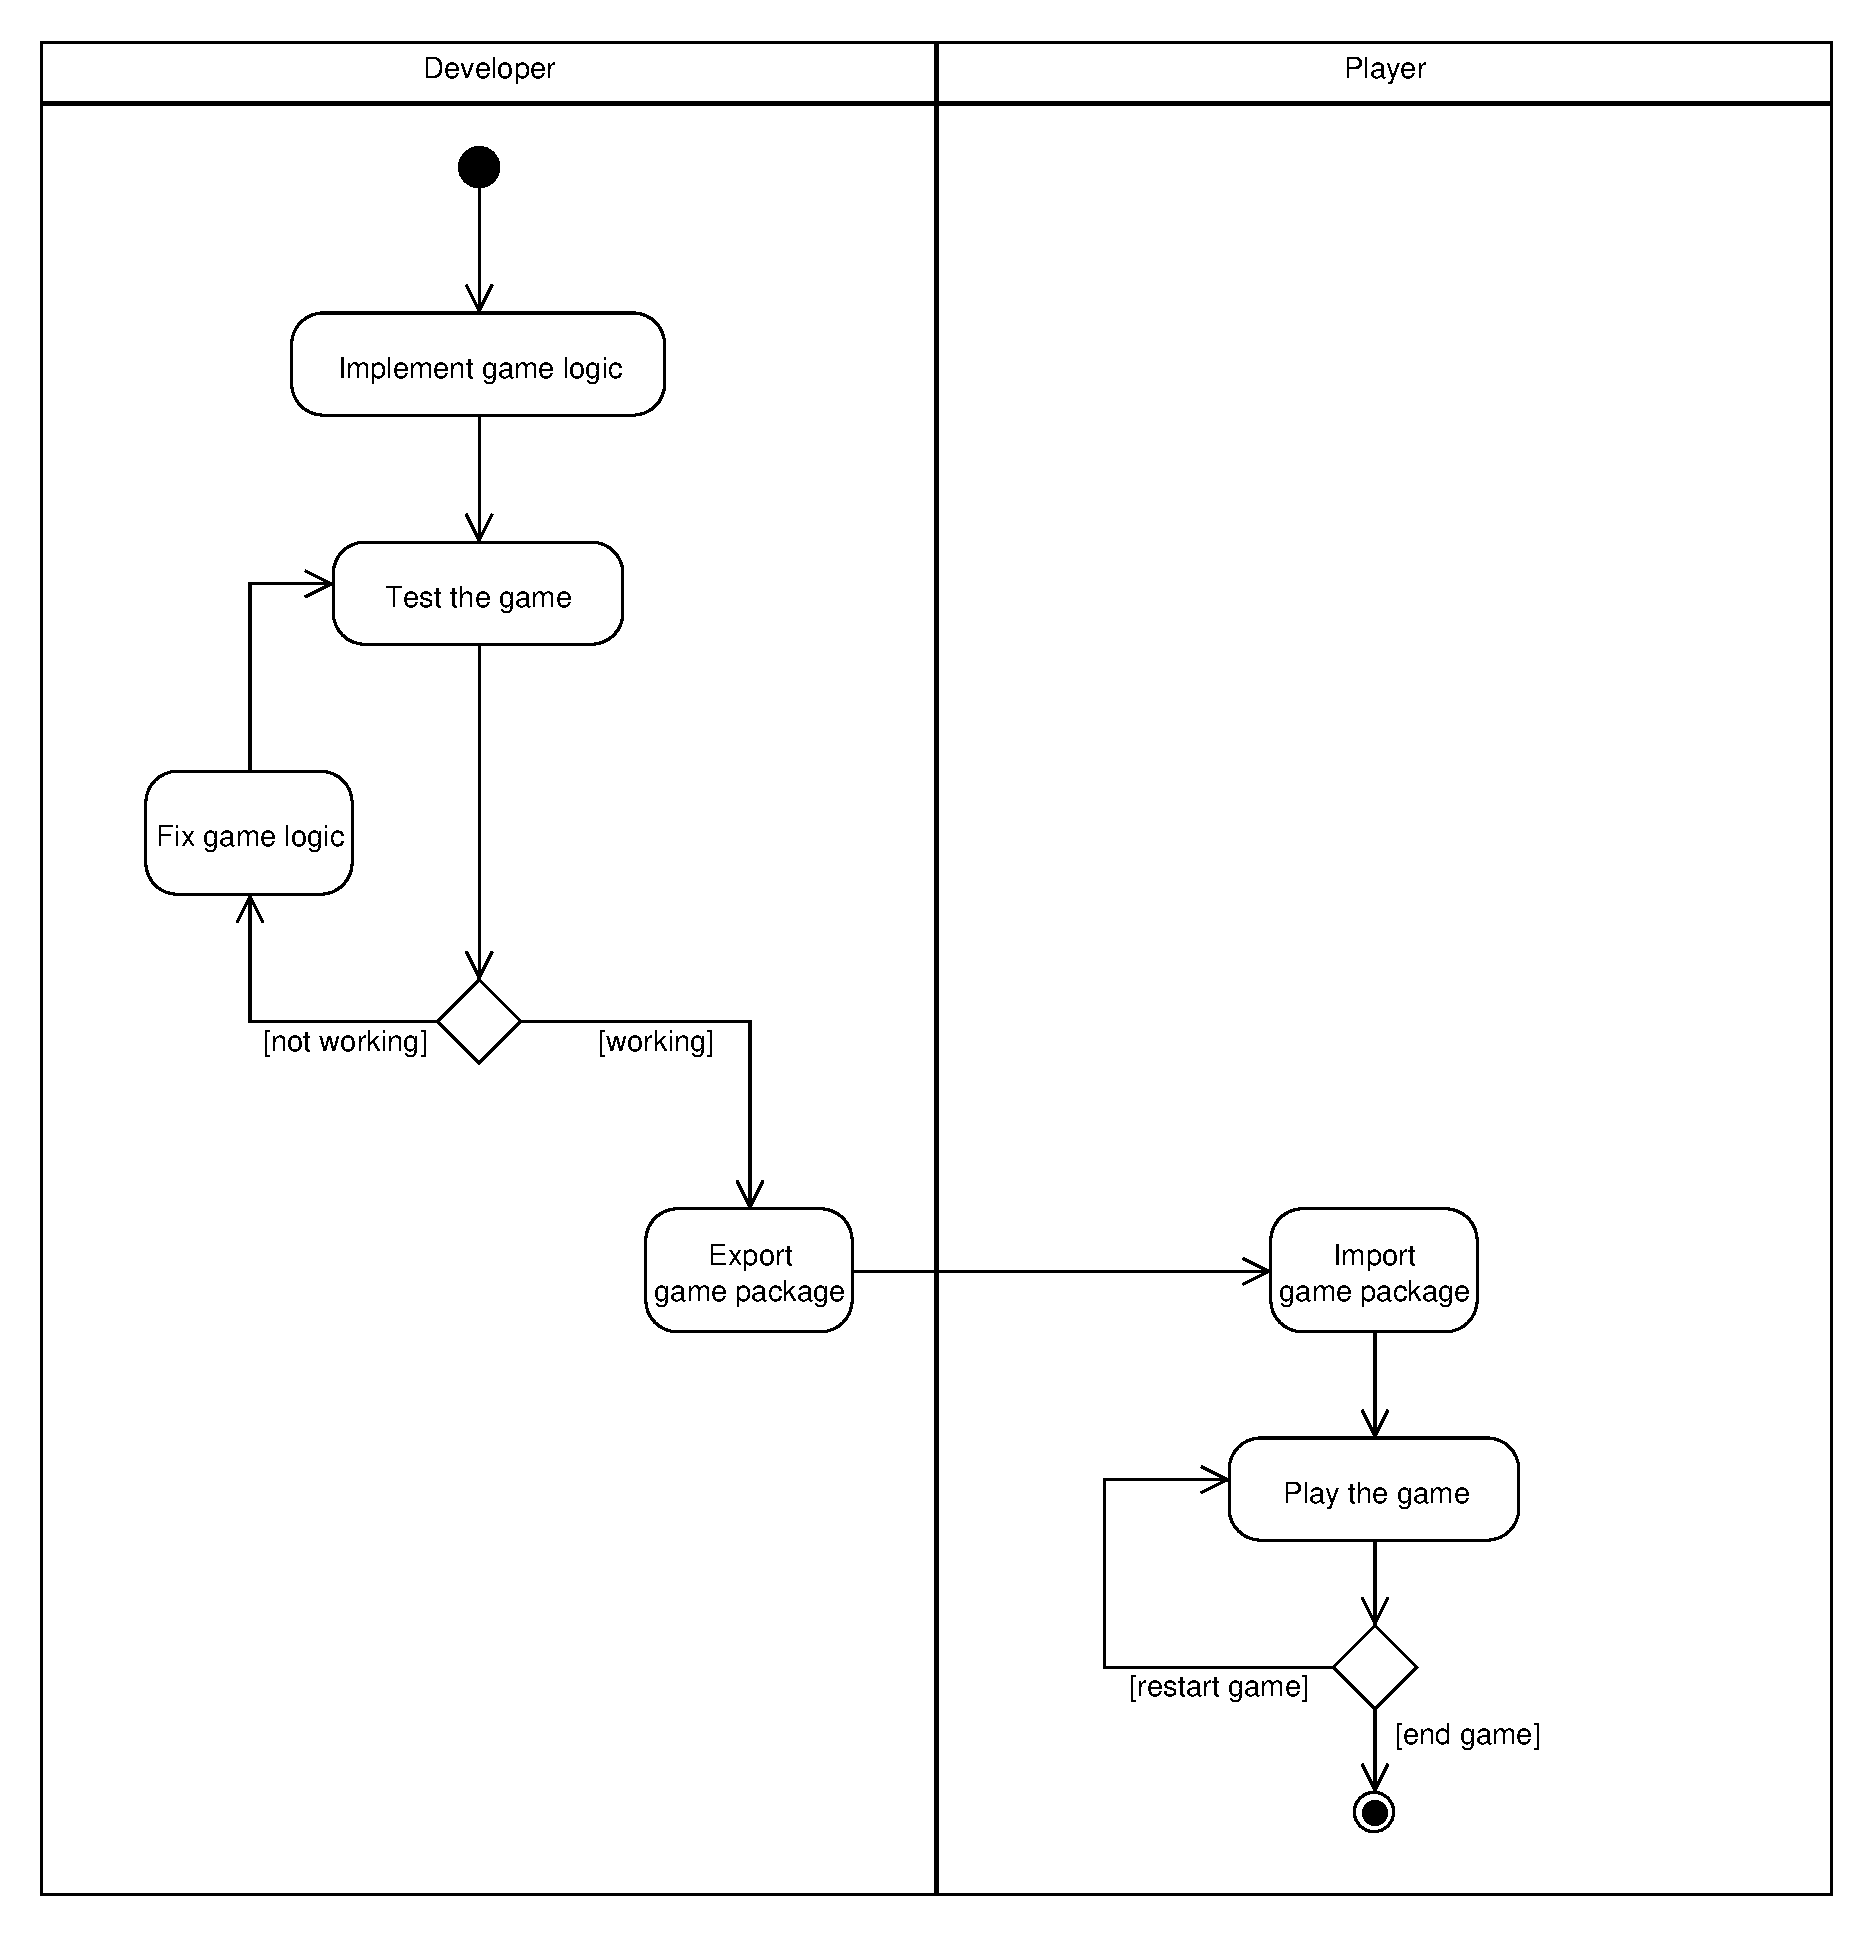
\includegraphics[width=\textwidth]{act_dev.pdf}
	\caption{Activity diagram showing the usual workflow of developing and using a game.}
	\label{img:ACTDEV}
\end{figure}
\subsubsection{Game: Graph-Coloring (Singleplayer)}
\begin{figure}[h!]
	\centering
	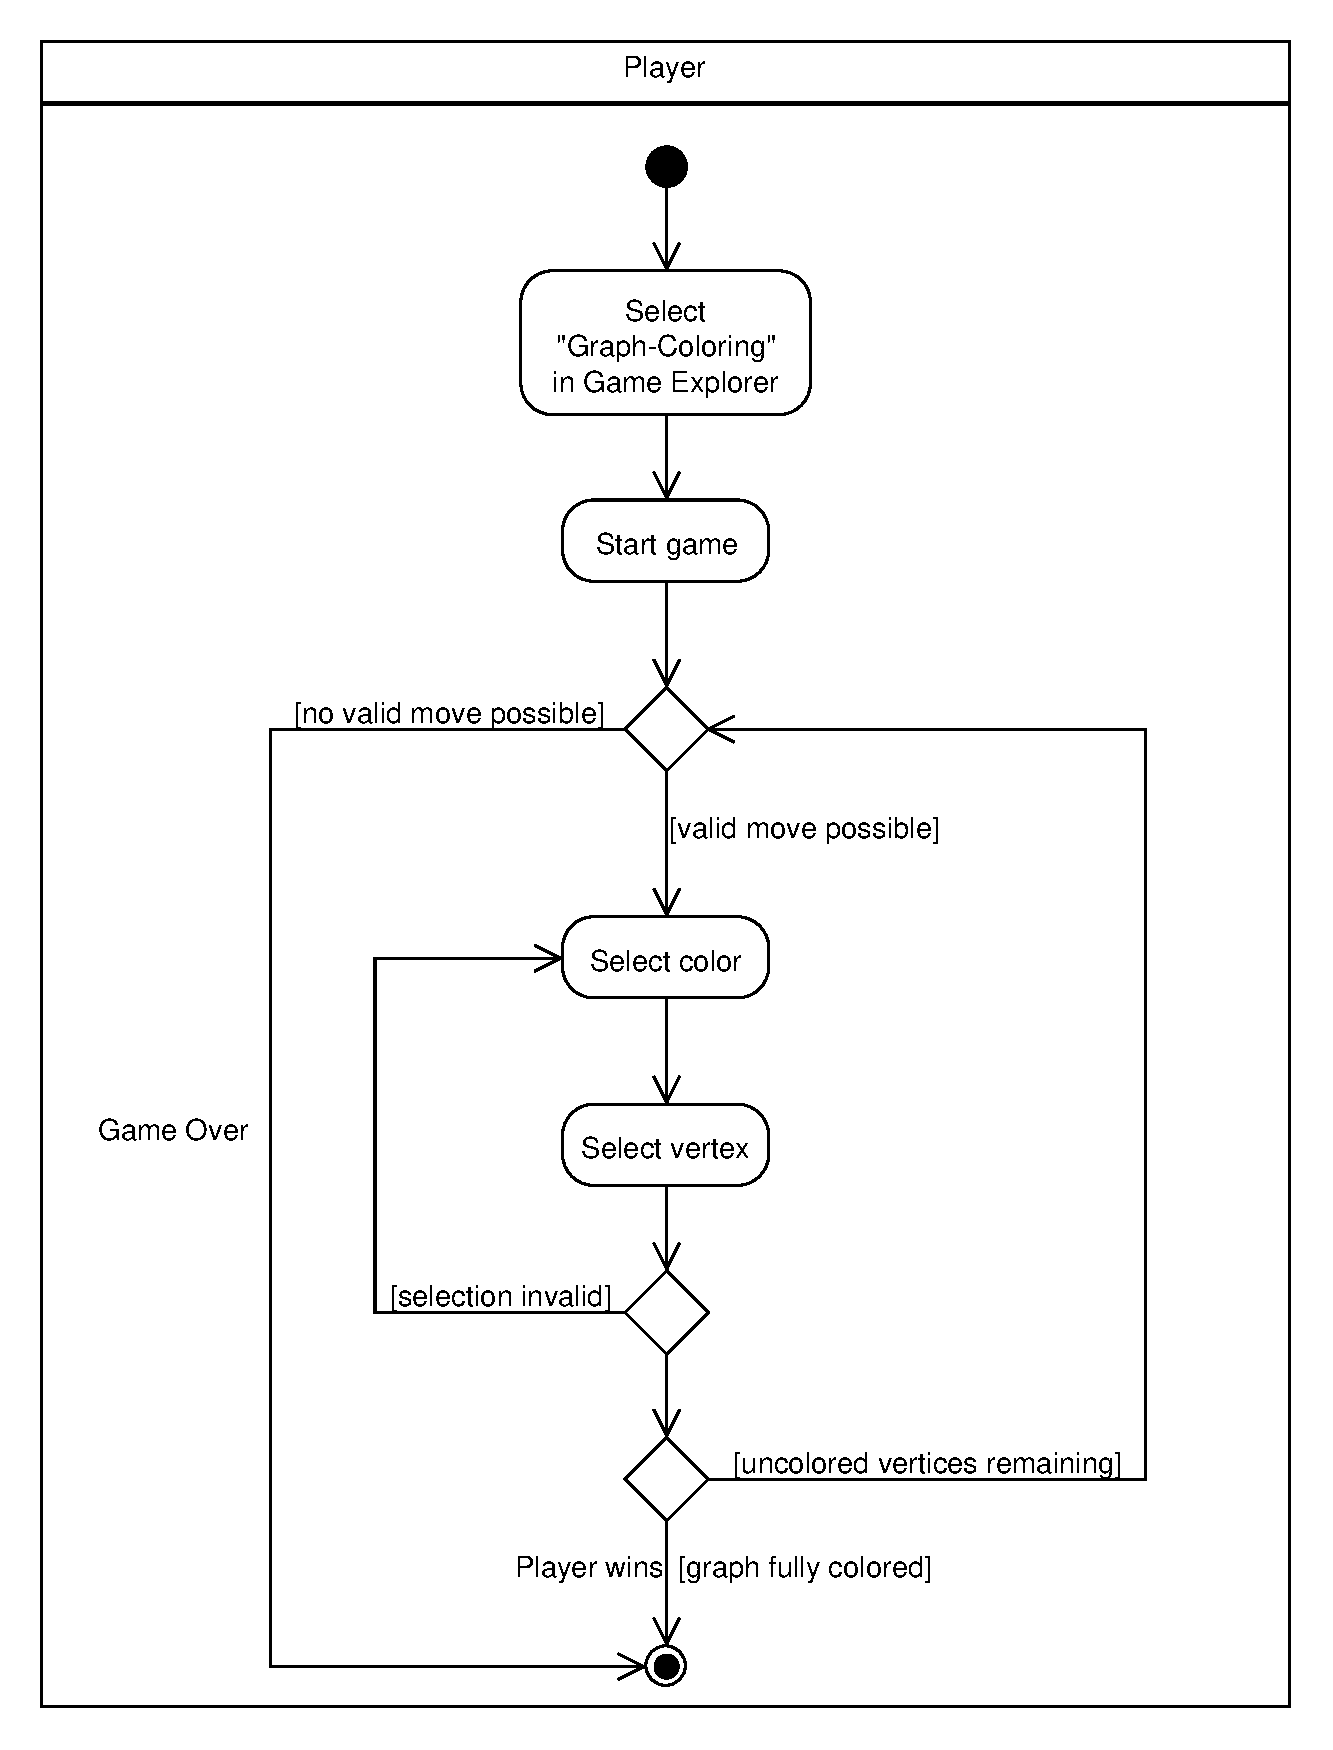
\includegraphics[width=\textwidth]{act_gc.pdf}
	\caption{Activity diagram of a game of 'Graph-Coloring (Singleplayer)'}
	\label{img:ACTGC}
\end{figure}
\section{Product performance}

%%%%%%%%%%% Framework %%%%%%%%%%%

\subsection{Framework}
\begin{tabular}{{c}{l}}
    \hline
    {\bf  Performance} & {\bf Description} \\ \hline
	\ref{PP:FW010} & \ref{PP:FWT010} \\
	\ref{PP:FW020} & \ref{PP:FWT020} \\
	\ref{PP:FW030} & \ref{PP:FWT030} \\	\hline
\end{tabular}

\vspace{.5cm}

\begin{description}
	\item[\textlabel{/PP010/}{PP:FW010}] \textbf{\textlabel{Maximum vertex/edge count}{PP:FWT010}} \\
	The framework must be able to handle at least 100 vertices and 300 edges in a single instance of a game.
	\item[\textlabel{/PP020/}{PP:FW020}] \textbf{\textlabel{Maximum player count}{PP:FWT020}} \\
	Up to four players should be able to participate in a game.
	\item[\textlabel{/PP030/}{PP:FW030}] \textbf{\textlabel{UI response time}{PP:FWT030}} \\
	The graphical user interface has to respond to user input within 0.3 seconds.
	
\end{description}

%%%%%%%%%%% Games %%%%%%%%%%%

\subsection{Implemented Games}

\begin{tabular}{{c}{l}}
    \hline
    {\bf Functions} & {\bf Description} \\ \hline
	\ref{PP:IG010} & \ref{PP:IGT010} \\ 
	\ref{PP:IG020} & \ref{PP:IGT020} \\ \hline
\end{tabular}

\vspace{.5cm}

\begin{description}
	\item[\textlabel{/PP040/}{PP:IG010}] \textbf{\textlabel{Validation}{PP:IGT010}} \\
	The games {\twixt} and {\graphcoloring} must not accept any invalid move by the player.
	\item[\textlabel{/PP050/}{PP:IG020}] \textbf{\textlabel{Short loading time}{PP:IGT020}} \\
	The loading time of the implemented games will be shorter than 5 seconds. \\
\end{description}
\section{Graphical User Interface}
\subsection{Game Explorer}

\begin{figure}[h]
	\centering
	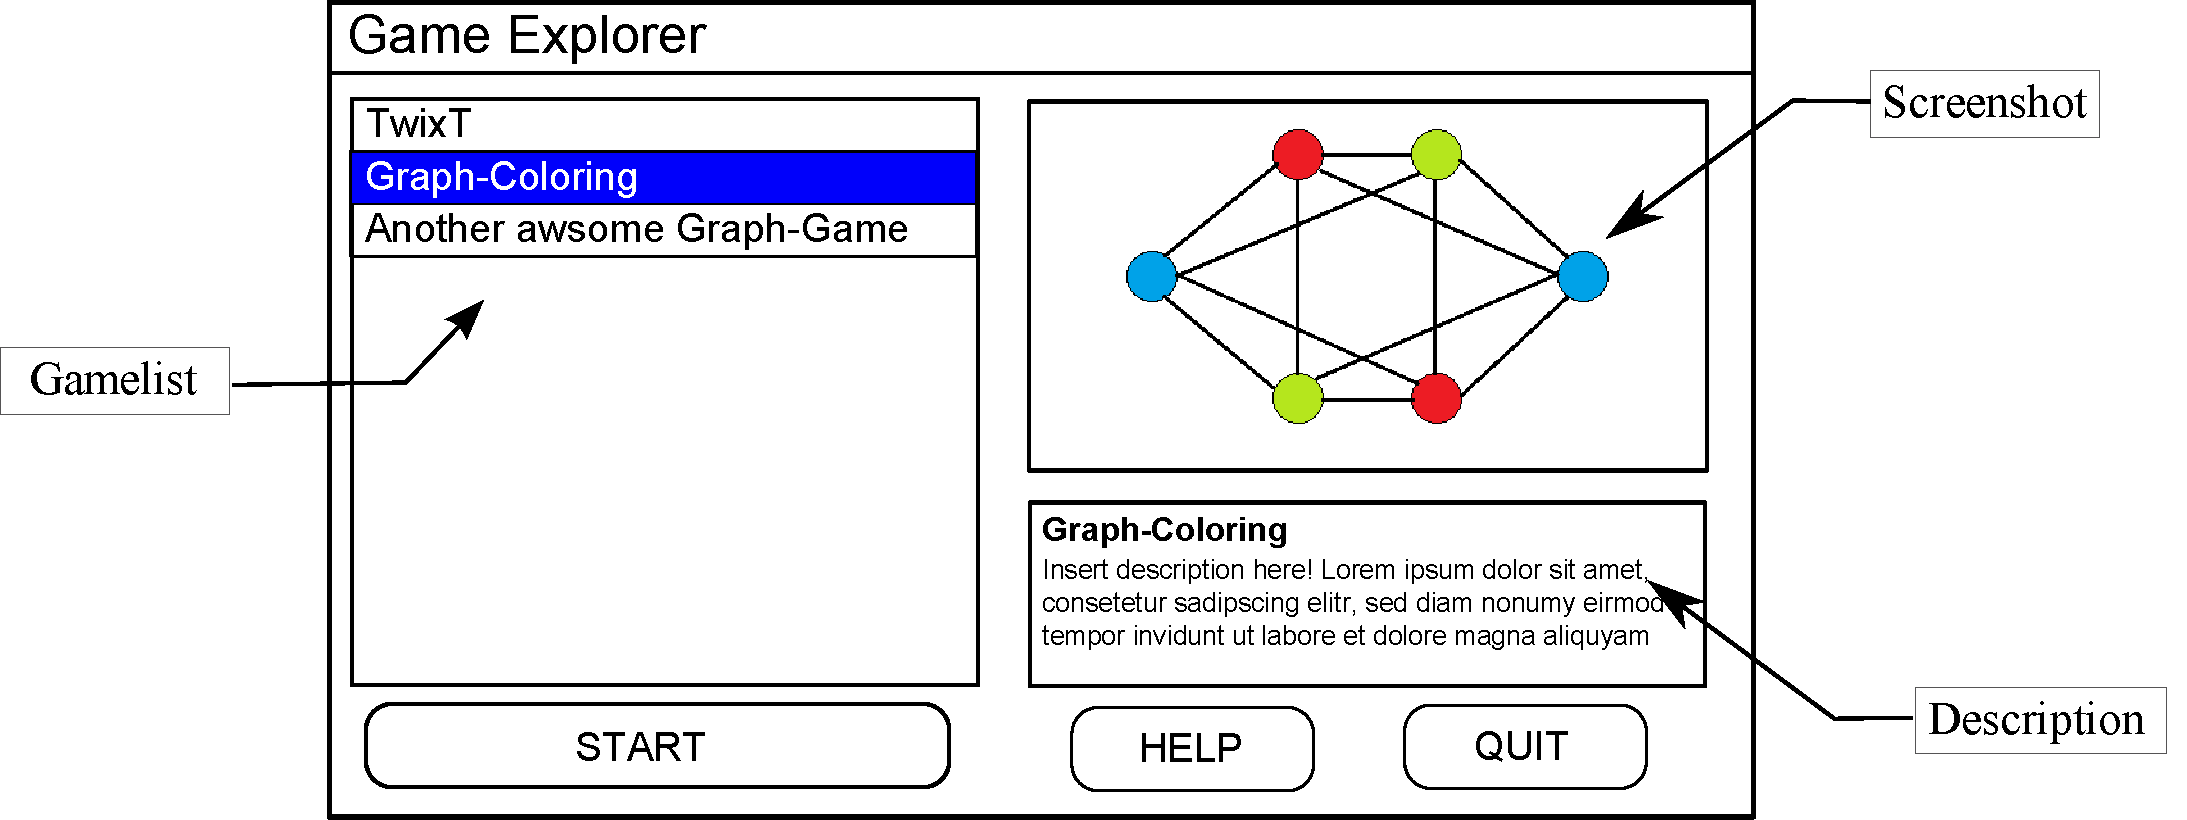
\includegraphics[max width=\linewidth]{gui_ge.pdf}
	\caption{Sketch of the Game Expolrer's GUI}
	\label{img:GE_GUI}
\end{figure}

\begin{description}
	\item[Gamelist] Displays a list of available Games and is used to select the game the user wants to play.
	\item[Screenshot] Shows a screenshot of the game currently selected.
	\item[Description] Shows a brief description of the game currently selected.
\end{description}

\subsection{Game}

\begin{figure}[H]
	\centering
	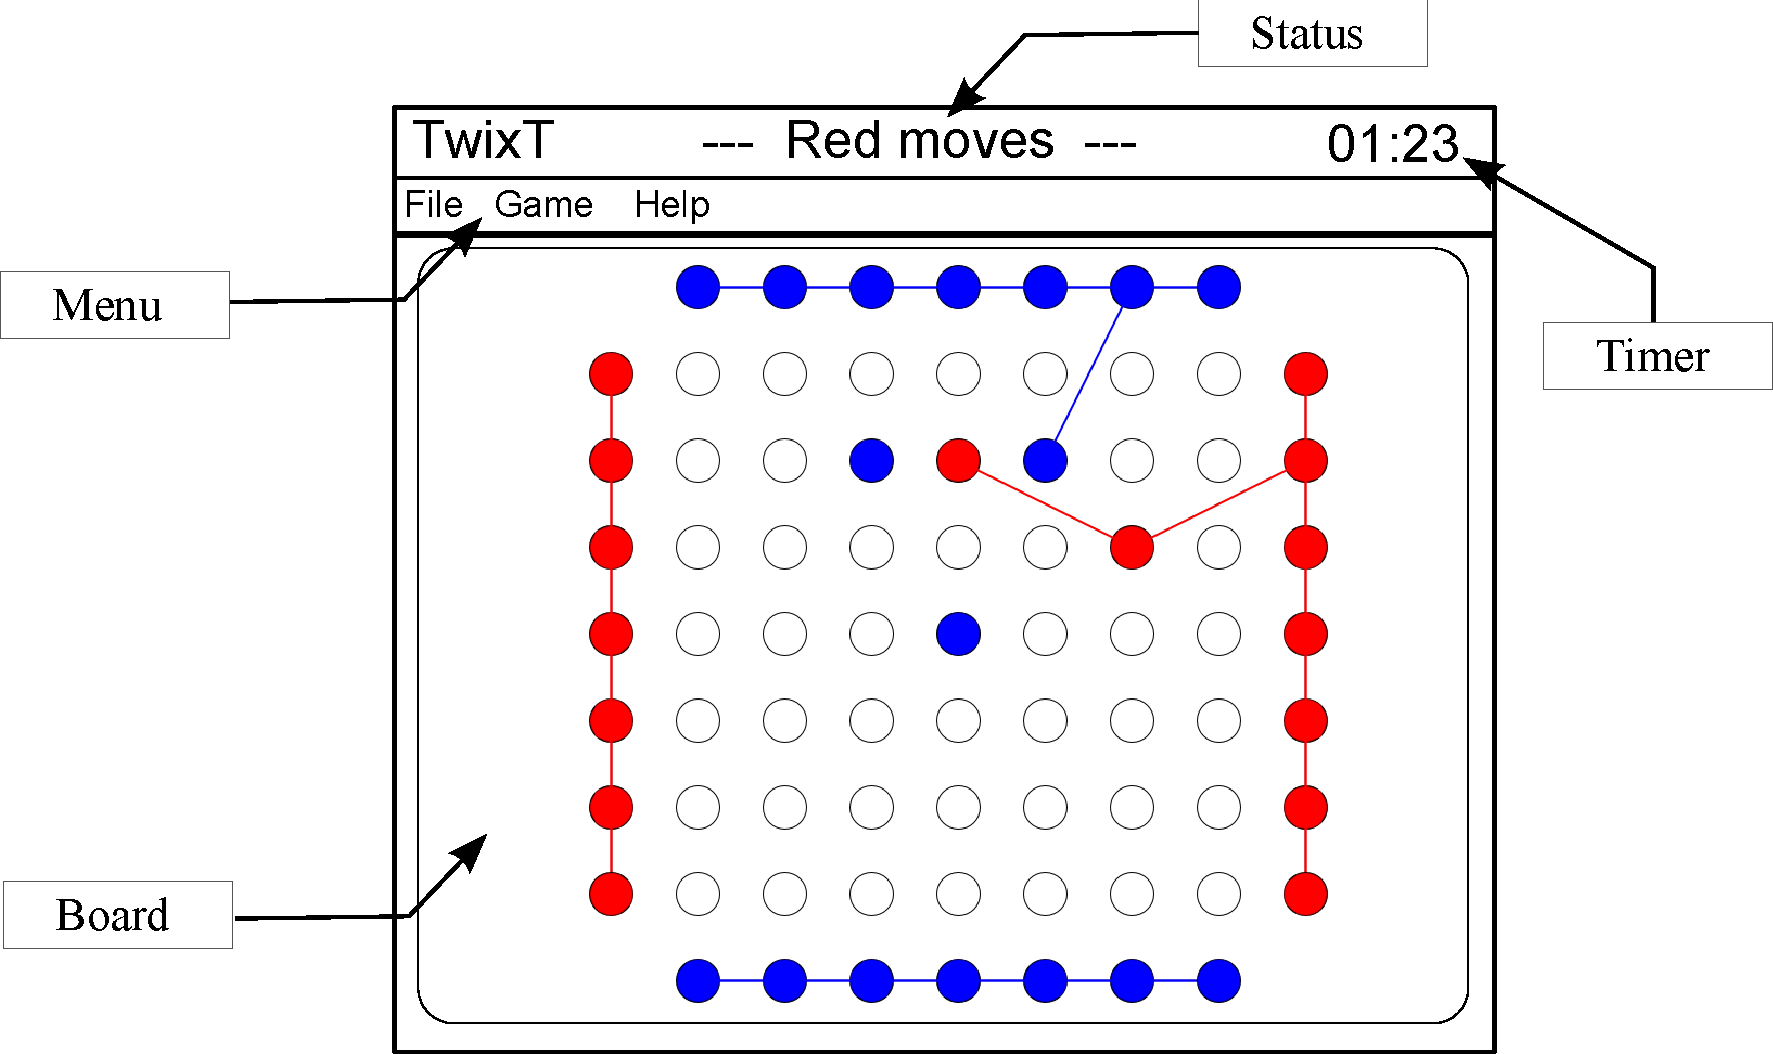
\includegraphics[max width=\linewidth]{gui_game.pdf}
	\caption{Sketch of a game's (TwixT) GUI}
	\label{img:GAME_GUI}
\end{figure}

\begin{description}
	\item[Board] Panel where the game's graph is displayed and the main part of the user interaction takes place.
	\item[Status] Gives short information about the game's status.
	\item[Menu] The game's menu.
\end{description}

\subsubsection{File}
\begin{description}
	\item[Restart] Starts the game from beginning.
	\item[Load] Load a previously saved game.
	\item[Save] Saves the state of the current game.
	\item[Exit] Closes the current game.
\end{description}
\subsubsection{Game}
This menu contains game specific options specified by the developer.
\subsubsection{Help}
\begin{description}
	\item[How to play] Shows an explanation of the current game.
	\item[About] Shows information about the current game and the framework,.
\end{description}





\section{Quality objective}

\begin{tabular}{lcccc}
\hline
\textbf{Criteria} & \textbf{very important} & \textbf{important} & \textbf{less important} & \textbf{least important} \\
	\hline
	Usability & $\times$ & & & \\
	Portability & $\times$ & & & \\
	Maintainability & $\times$ & & & \\
	Reliability & & $\times$ & & \\
	Consistency & & $\times$ & & \\
	Efficiency & & & $\times$ & \\
	Security & & & & $\times$ \\
	\hline
\end{tabular}


\begin{description}
	\item[Usability] Ease of use of the framework.
	\item[Portability] Capability of the framework to run in different environments and amount of effort it takes to adapt it to new environments.
	\item[Maintainability] The degree of effort required to correct software defects and to cope with user complaints\footnote{Fenton, Norman E.; Pfleeger, Shari L.: Software Metrics: A Rigorous and Practical Approach (1997)}.
	\item[Reliability] Ability of the framework to perform its functions without failure in normal and stress situations.
	\item[Consistency] Those attributes of the framework that provide uniform design and implementation techniques and notations.\footnote{McCall, J. A.; Richards, P. K., Walters, G. F.: Factors in Software Quality (1977)}
	\item[Efficiency] Ratio of the complexity of a task to the effort (time, memory space) necessary to achieve it.
	\item[Security] Level of protection against potential security breaches.
	
\end{description}
\section{Test cases}
\subsection{Game-Explorer}

\begin{tabular}{cll}
	\hline
	\textbf{Test} & \textbf{Description} & \textbf{Tested Functionalities} \\
	\hline
	\ref{T:010} & \ref{T:010T} & \ref{FR:GE010}, \ref{FR:GE020} \\
	\ref{T:020} & \ref{T:020T} & \ref{FR:GE050} \\
	\ref{T:030} & \ref{T:030T} & \ref{FR:GE030} \\
	\ref{T:040} & \ref{T:040T} & \ref{FR:GE040} \\
	\hline
\end{tabular}

\begin{description}
	\item[\textlabel{/T010/}{T:010}] \textbf{\textlabel{Start the Game-Explorer}{T:010T}} \\
	\textbf{Input:} The tester clicks the Game-Explorer icon. \\
	\textbf{Exp. Output:} The Game-Explorer window opens, the game folder is scanned and all games contained are shown in the games list.
	
	\item[\textlabel{/T020/}{T:020}] \textbf{\textlabel{Select a game}{T:020T}} \\
	\textbf{Input:} The tester clicks on the name of the game in the list. \\
	\textbf{Exp. Output:} An image and a description of the game are displayed.
	
	\item[\textlabel{/T030/}{T:030}] \textbf{\textlabel{Start a game}{T:030T}} \\
	\textbf{Input:} A game has been selected and the tester clicks on the start button. \\
	\textbf{Exp. Output:} The game window opens.
	
	\item[\textlabel{/T040/}{T:040}] \textbf{\textlabel{Use the help function}{T:040T}} \\
	\textbf{Input:} A game has been selected and the tester clicks on the help button. \\
	\textbf{Exp. Output:} The help page is displayed in a new window.
\end{description}

\subsection{Games}
\subsubsection\graphcoloring

\begin{tabular}{cll}
	\hline
	\textbf{Test} & \textbf{Description} & \textbf{Tested Functionalities} \\
	\hline
	\ref{T:050} & \ref{T:050T} & \ref{FR:L010}, \ref{FR:L020},\ref{FR:GU010}, \\
	 & & \ref{FR:GU020} \\
	\ref{T:060} & \ref{T:060T} & \ref{FR:G010}, \ref{FR:G020}\\
	\ref{T:070} & \ref{T:070T} & \ref{FR:L040}, \ref{FR:L050}, \ref{FR:GU030} \\
	\ref{T:080} & \ref{T:080T} & \ref{FR:L040}, \ref{FR:L050}, \ref{FR:GU030}\\
	\ref{T:090} & \ref{T:090T} & \ref{FR:L040}, \ref{FR:L050}, \ref{FR:L100}, \\
	 & & \ref{FR:GU030}, \ref{FR:GU040}\\
	\ref{T:100} & \ref{T:100T} & \ref{FR:L100}, \ref{FR:GU040} \\
	\hline
\end{tabular}

\todo{add testcase for multiplayer}

\begin{description}
	\item[\textlabel{/T050/}{T:050}] \textbf{\textlabel{Start the game}{T:050T}} \\
	\textbf{Input:} \graphcoloring has been selected and the tester clicks on the start button. \\
	\textbf{Exp. Output:} The game window opens and the graph of the first level is displayed.
	
	\item[\textlabel{/T060/}{T:060}] \textbf{\textlabel{Save and load a game}{T:060T}} \\
	\textbf{Input:} Some vertices have been colored. The tester saves the current state, closes and reopens \graphcoloring and loads the savegame. \\
	\textbf{Exp. Output:} The state is saved in a file and when the file is loaded, the saved state is restored.
	
	\item[\textlabel{/T070/}{T:070}] \textbf{\textlabel{Color an uncolored vertex}{T:070T}} \\
	\textbf{Input:} The tester selects a color and clicks on an uncolored vertex that is not adjacent to one in the same color. \\
	\textbf{Exp. Output:} The vertex changes its color to the selected one.
	
	\item[\textlabel{/T080/}{T:080}] \textbf{\textlabel{Color a colored vertex}{T:080T}} \\
	\textbf{Input:} The tester selects a color and clicks on a colored vertex. \\
	\textbf{Exp. Output:} Nothing changes.
	
	\item[\textlabel{/T090/}{T:090}] \textbf{\textlabel{Color adjacent vertices in the same color}{T:090T}} \\
	\textbf{Input:} The tester selects a color and clicks on an uncolored vertex that is adjacent to one in the same color. \\
	\textbf{Exp. Output:} The vertex does not change. An error message is displayed.
	
	\item[\textlabel{/T100/}{T:100}] \textbf{\textlabel{Win/Lose a game}{T:100T}} \\
	\textbf{Input:} The tester plays until he won/lost the game. \\
	\textbf{Exp. Output:} A win/lose message is displayed and the next/same level is loaded.
\end{description}

\subsubsection\twixt

\begin{tabular}{cll}

\hline
	\textbf{Test} & \textbf{Description} & \textbf{Tested Functionalities} \\
	\hline
	\ref{T:110} & \ref{T:110T} & \ref{FR:L010}, \ref{FR:L020},\ref{FR:GU010} \\
	\ref{T:120} & \ref{T:120T} & \ref{FR:G010}, \ref{FR:G020} \\
	\ref{T:130} & \ref{T:130T} & \ref{FR:L030}, \ref{FR:L040}, \ref{FR:L100}, \\
	 & & \ref{FR:GU040} \\
	\ref{T:140} & \ref{T:140T} & \ref{FR:L030}, \ref{FR:L040}, \ref{FR:L050}, \\
	 & & \ref{FR:L100},  \ref{FR:GU040} \\
	\ref{T:150} & \ref{T:150T} & \ref{FR:L030}, \ref{FR:L040} \\
	\ref{T:160} & \ref{T:160T} & \ref{FR:L060}, \ref{FR:L070} , \ref{FR:L100}, \\
	& & \ref{FR:GU040} \\
	\hline
\end{tabular}

\todo{add test case "connecting vertices of wrong distance"}

\begin{description}
	\item[\textlabel{/T110/}{T:110}] \textbf{\textlabel{Start the game}{T:110T}} \\
	\textbf{Input:} \twixt has been selected and the tester clicks on the start button. \\
	\textbf{Exp. Output:} The game window opens and the empty grid is displayed.
	
	\item[\textlabel{/T120/}{T:120}] \textbf{\textlabel{Save and load a game}{T:120T}} \\
	\textbf{Input:} Some vertices have been placed. The tester saves the current state, closes and reopens \twixt and loads the savegame. \\
	\textbf{Exp. Output:} The state is saved in a file and when the file is loaded, the saved state is restored.
	
	\item[\textlabel{/T130/}{T:130}] \textbf{\textlabel{Place edges and vertices}{T:130T}} \\
	\textbf{Input:} The tester places vertices and connects them with edges for both players without intersection. \\
	\textbf{Exp. Output:} The placed vertices and edges are displayed. Each turn the status displays which player's turn it is.
	
	\item[\textlabel{/T140/}{T:140}] \textbf{\textlabel{Place an edge across another one}{T:140T}} \\
	\textbf{Input:} Two vertices have been connected by an edge. The tester clicks on two other vertices on either side of the edge. \\
	\textbf{Exp. Output:} The vertices do not get connected. An error message is displayed.
	
	\item[\textlabel{/T150/}{T:150}] \textbf{\textlabel{Place a vertex on an already occupied field}{T:150T}} \\
	\textbf{Input:} A vertex has been placed. The tester clicks the vertex again. \\
	\textbf{Exp. Output:} Nothing changes.
	
	\item[\textlabel{/T160/}{T:160}] \textbf{\textlabel{Win/Lose a game}{T:160T}} \\
	\textbf{Input:} The tester plays for both players until one won the game. \\
	\textbf{Exp. Output:} A win message for the winning player is displayed.
\end{description}

\subsection{Test scenarios}

\subsubsection{Use the Game-Explorer}

Alice starts the Game-Explorer and selects \graphcoloring in the list in order to look at the screenshot and the description of the game. Still not convinced, Alice uses the help function to gain an insight in how \graphcoloring works. Then Alice starts the game.

\subsubsection{Play \graphcoloring single-player} \label{T:GCSingle}

Bob starts \graphcoloring with the Game-Explorer. Bob selects the color red and colors vertex 1. Then Bob selects blue, colors vertex 3 and 4 and tries to color vertex 2, but it stays uncolored. The status bar displays an error message for a few seconds. Bob then selects green and colors vertex 2. A win message is displayed. Then Bob closes the game.

\subsubsection{Play \graphcoloring multiplayer} \label{T:GCMulti}

Carol and Dave start \graphcoloring with the Game-Explorer. Carol selects the color blue and colors vertex 2. Dave selects red and colors vertex 4. Carol selects green and tries to color vertex 2, but it stays blue. Carol then colors vertex 3. Since no valid move is possible anymore, a win message for Carol is displayed. Dave then closes the game.

\begin{figure}[h!]
	\centering
	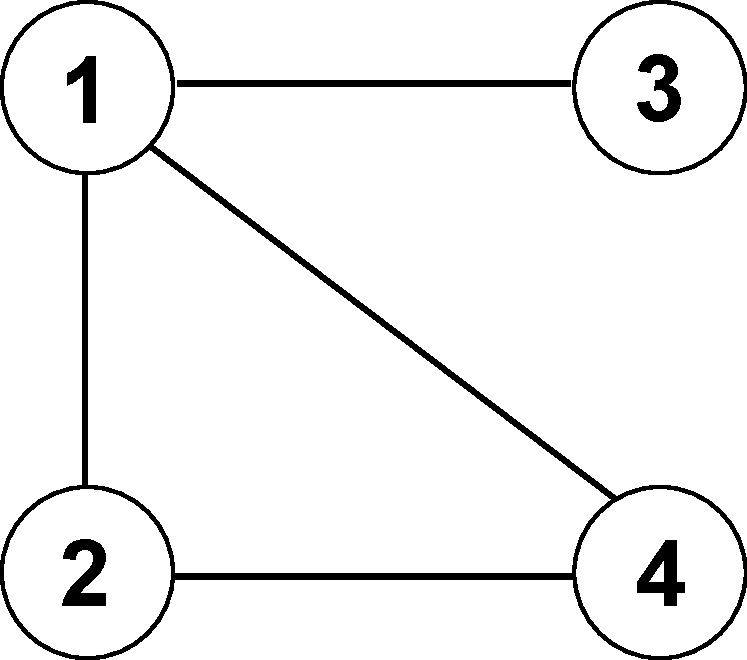
\includegraphics[width=0.25\textwidth]{testgraph.pdf}
	\caption{Graph the scenarios \ref{T:GCSingle} and \ref{T:GCMulti} are based on}
	\label{img:ACTDEV}
\end{figure}

\subsubsection{Play \twixt} \label{T:TwixT}

Carol and Dave start \twixt with the Game-Explorer. They select a 7$\times$7 grid and the grid is displayed. Dave starts and places a vertex on position C3. Carol places a vertex on position E3. Dave places a vertex on position E4. Carol places a vertex on position D5. Dave connects his placed vertices with an edge. Carol also tries to connect the vertices she placed. The status bar displays an error message for a few seconds. Carol then places a vertex on position F5. Dave connects the vertex on C3 with the vertex of his left border row on position A4. Carol tries to place a vertex on position C3, but it does not change. Carol then connects the vertex on E3 with her upper border row on position F1. Dave closes his path by connecting his vertex on E4 with his right border row on position G3. A win message for Dave is displayed. Dave then closes the game.

\begin{figure}[h!]
	\centering
	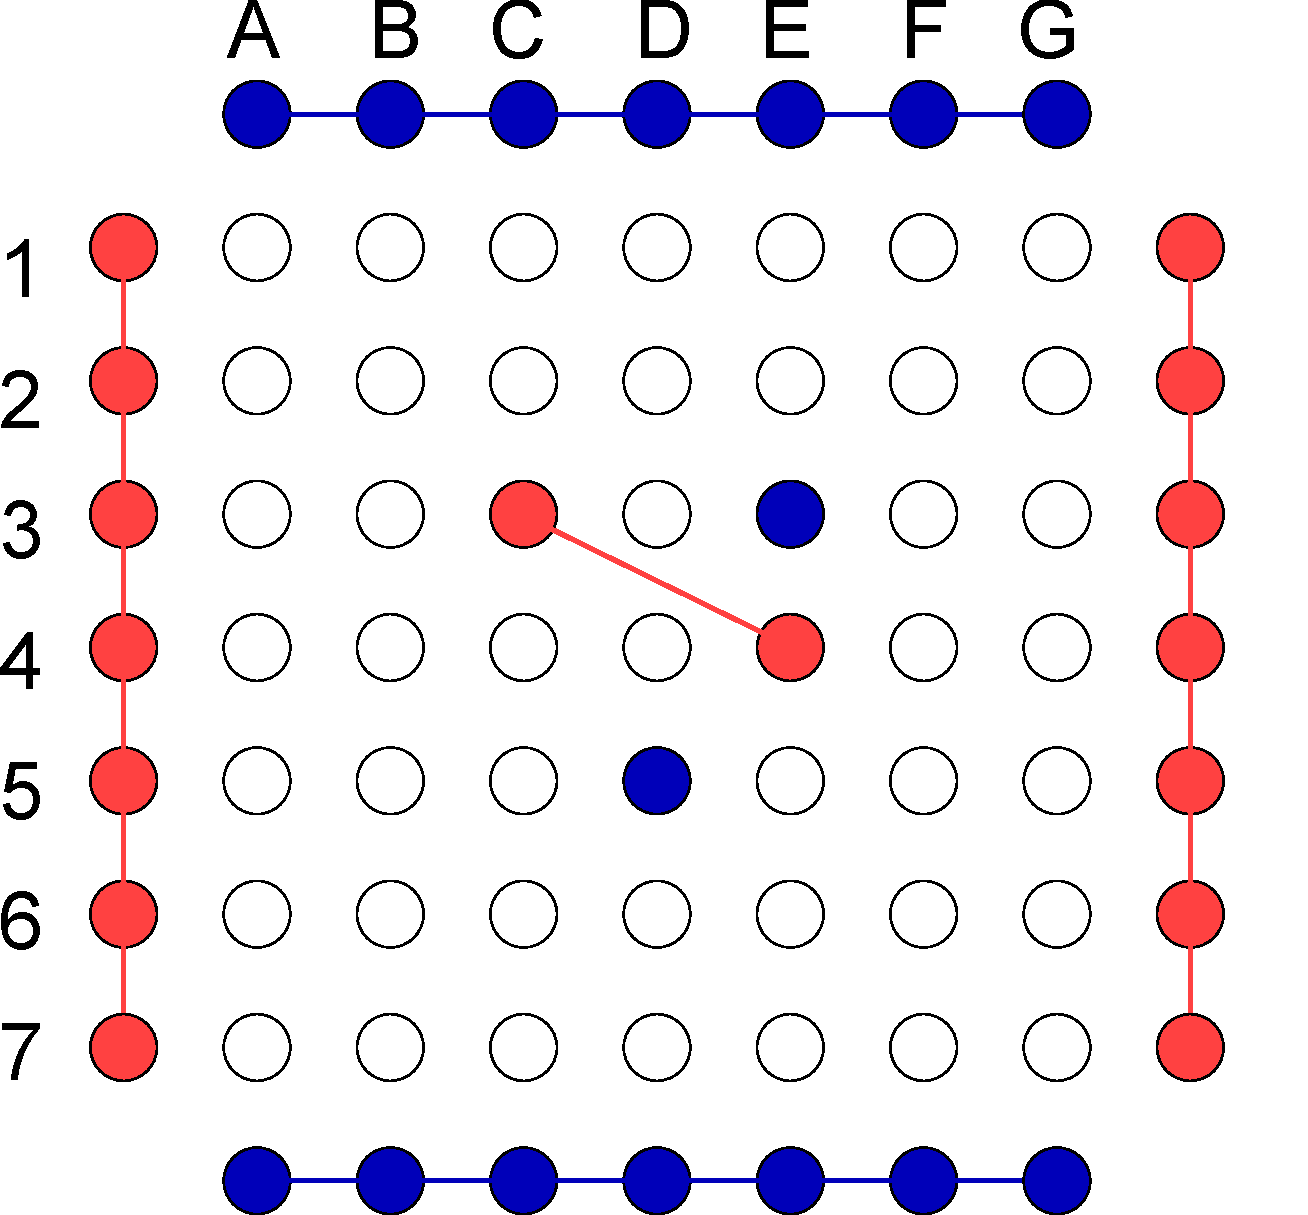
\includegraphics[width=0.35\textwidth]{testtwixt.pdf}
	\caption{Scenario \ref{T:TwixT} after Dave's (red) third move}
	\label{img:ACTDEV}
\end{figure}
\section{Development environment}

The framework will be implemented using the Eclipse Java IDE with the JVM version 1.6.31 and the Git revision control system. For testing purposes the JUnit Testing Framework will be used.
\section{Glossary}

\end{document}